\documentclass{beamer}
\usepackage[utf8]{inputenc}
\usepackage[UKenglish]{babel}
\usepackage[UKenglish]{isodate}
\usepackage{mathtools}
\usepackage{tikz}
\usepackage{microtype}
\usepackage{complexity}
\usepackage{forest}
\usepackage[style=authoryear]{biblatex}
\usepackage{soul}

\usetikzlibrary{shapes}
\usetikzlibrary{positioning}
\usetikzlibrary{overlay-beamer-styles}
\usetikzlibrary{shapes.callouts}
\usetikzlibrary{cd}
\usetikzlibrary{calc}
\usetikzlibrary{backgrounds}
\usetikzlibrary{fit}
\usetikzlibrary{decorations.pathreplacing}

\forestset{
sn edges/.style={for tree={edge={-Latex}}},
  visible on/.style={
    for tree={
      /tikz/visible on={#1},
      edge+={/tikz/visible on={#1}}}}
}

\beamertemplatenavigationsymbolsempty
\usetheme{default}
\usecolortheme{rose}

\definecolor{color1}{HTML}{1B9E77}
\definecolor{color2}{HTML}{7570b3}

\newcommand{\pP}{\texttt{P}}
\newcommand{\qQ}{\texttt{Q}}
\DeclareMathOperator{\GDR}{\textsc{GDR}}
\DeclareMathOperator{\CR}{\textsc{CR}}
\DeclareMathOperator{\Reff}{\textsc{Ref}}

\addbibresource{talk.bib}

\author{\textbf{Paulius Dilkas}\inst{1} \and Vaishak Belle\inst{2}}
\title{Synthesising Recursive Functions for\\First-Order Model Counting:}
\subtitle{Challenges, Progress, and Conjectures}
\institute{\inst{1}National University of Singapore, Singapore \and \inst{2}University of Edinburgh, UK}
\date{KR 2023}

\begin{document}
\addtobeamertemplate{block begin}{\setlength\abovedisplayskip{0pt}}

\begin{frame}[noframenumbering,plain]
  \tikz[remember picture,overlay]{
    \node at ([yshift=20pt,xshift=-20pt]current page.south)
    {
\includegraphics[height=40pt]{nus.jpg}};
    \node at ([yshift=25pt,xshift=30pt]current page.south)
    {
\includegraphics[height=40pt]{inf.png}};
    \node at ([yshift=25pt,xshift=75pt]current page.south)
    {
\includegraphics[height=40pt]{ecr.jpg}};
    \node at ([yshift=20pt,xshift=140pt]current page.south)
    {
\includegraphics[height=20pt]{epsrc.png}};
  }
  \titlepage
\end{frame}

\begin{frame}{Some Elementary Counting}
  \begin{exampleblock}{A Counting Problem}
    Suppose this room has \structure{$n$} seats, and there are
    \structure{$m \le n$} people in the audience. How many ways are there to
    seat everyone?
  \end{exampleblock}

  \pause
  More explicitly, we assume that:
  \begin{itemize}
  \item each attendee gets exactly one seat,
  \item and a seat can accommodate at most one person.
  \end{itemize}

  \pause
  \alert{Answer:} \structure{$n^{\underline{m}} = n \cdot (n-1)\cdots(n-m+1)$}.

  Note: this problem is equivalent to counting \structure{$[m] \to [n]$} injections.

\end{frame}
% wouldn't it be nice if we could just describe this problem and have an
% algorithm solve it for us?

\begin{frame}{Let's Express This Problem in Logic!}
  \begin{itemize}
    \item Let \structure{$\Gamma$} and \structure{$\Delta$} be sets (i.e.,
    \alert{domains})
          \begin{itemize}
            \item such that \structure{$|\Gamma| = m$}, and
                  \structure{$|\Delta| = n$}
          \end{itemize}
    \item Let \structure{$\pP{} \subseteq \Gamma \times \Delta$} be a relation
          (i.e., \alert{predicate}) over \structure{$\Gamma$} and
          \structure{$\Delta$}
    \item We can describe all of the constraints in first-order logic:
          \begin{itemize}
            \item \pause each attendee gets a seat (i.e., at least one seat)
                  \begin{equation}\label{eq1}
                    \forall x \in \Gamma\text{. }\exists y \in \Delta\text{. }\pP{}(x, y)
                  \end{equation}
            \item \pause one person cannot occupy multiple seats
                  \begin{equation}\label{eq2}
                    \forall x \in \Gamma\text{. }\forall y, z \in \Delta\text{. }\pP{}(x, y) \land \pP{}(x, z) \Rightarrow y=z
                  \end{equation}
            \item \pause one seat cannot accommodate multiple attendees
                  \begin{equation}\label{eq3}
                    \forall w, x \in \Gamma\text{. }\forall y \in \Delta\text{. }\pP{}(w, y) \land \pP{}(x, y) \Rightarrow w=x
                  \end{equation}
          \end{itemize}
  \end{itemize}
  \pause
  \alert{\eqref{eq1}} and \alert{\eqref{eq2}} constrain \structure{$\pP{}$} to be a function, and \alert{\eqref{eq3}} makes it injective.
\end{frame}
% one could also add probabilities to these sentences to say that, e.g., there is a 1% probability of somebody taking up two seats, somebody sitting on somebody else's lap, somebody sitting on the floor, etc.

\begin{frame}{Overview of the Problem}
  \begin{itemize}
    \item \alert{First-order model counting} (FOMC) is the problem of counting
          the models of a sentence in first-order logic.
    \item The \alert{(symmetric) weighted} variation of the problem adds weights
          (e.g., probabilities) to predicates.
          \begin{itemize}
            \item It is used for efficient \alert{probabilistic inference} in
                  relational models such as Markov logic networks.
          \end{itemize}
  \end{itemize}
  \begin{block}{Claim}
    The capabilities of FOMC algorithms can be expanded by enabling them to
    construct \alert{recursive solutions}.
  \end{block}
\end{frame}

\begin{frame}{Back to Our Example}
  The following function counts injections:
  \[
    f(m, n) =
    \begin{cases}
      1 & \text{if } m = 0 \text{ and } n = 0 \\
      0 & \text{if } m > 0 \text{ and } n = 0 \\
      f(m, n-1) + m \times f(m-1, n-1) & \text{otherwise.}
    \end{cases}
  \]
  \pause
  \begin{itemize}
    \item \structure{$f(m, n)$} can be computed in \structure{$\Theta(mn)$} time
          \begin{itemize}
            \item using dynamic programming.
          \end{itemize}
    \item \alert{Optimal} time complexity to compute
          \structure{$n^{\underline{m}}$} is \structure{$\Theta(m)$}.
    \item But \structure{$\Theta(mn)$} is still much better than translating to
          propositional logic and solving a \alert{$\#\P$-complete} problem.
    \item The rest of this talk is about how such functions can be found
          automatically.
  \end{itemize}
\end{frame}

\begin{frame}{First-Order Knowledge Compilation: Before and After}
  \begin{columns}[b]
    \begin{column}{0.4\textwidth}
      \centering
      \begin{tikzpicture}
        \node (start) {\tiny $\forall x \in \Delta\text{. } \pP(x) \lor \qQ(x)$};
        \node[draw,rounded rectangle,fill=color2!50,below=0.7cm of start] (kc) {Compilation};
        \node[below=0.7cm of kc] (graph) {
          \scalebox{.5}{
            \begin{forest}
              for tree={sn edges,fill=red!50,ellipse,draw}
              [[
              [
              []
              []
              ]
              [
              [
              []
              []
              ]
              []
              ]
              ]]
            \end{forest}
          }
        };
        \node[draw,rounded rectangle,fill=color2!50,below=0.7cm of graph] (evaluation) {Propagation};
        \node[below=0.7cm of evaluation] (end) {
\includegraphics[height=0.4cm]{81.png}};
        \node[right=0.3cm of evaluation] (sizes) {\tiny $|\Delta| = 4$};
        \draw[-Latex,color=color2] (start) -- (kc);
        \draw[-Latex,color=color2] (kc) -- (graph);
        \draw[-Latex,color=color2] (graph) -- (evaluation);
        \draw[-Latex,color=color2] (evaluation) -- (end);
        \draw[-Latex,color=color2] (sizes) -- (evaluation);
        \node[draw,fit={(kc) (graph) (evaluation)},inner xsep=1pt,inner ysep=2pt] {};
      \end{tikzpicture}
    \end{column}
    \pause
    \begin{column}{0.6\textwidth}
      \centering
      \begin{tikzpicture}
        \node (start) {\tiny $\begin{gathered}
            \forall x \in \Gamma\text{. }\exists y \in \Delta\text{. }\pP(x, y)\\
            \forall x \in \Gamma\text{. }\forall y, z \in \Delta\text{. }\pP(x, y) \land \pP(x, z) \Rightarrow y=z\\
            \forall w, x \in \Gamma\text{. }\forall y \in \Delta\text{. }\pP(w, y) \land \pP(x, y) \Rightarrow w=x
          \end{gathered}$};
        \node[draw,rounded rectangle,fill=color2!50,below=0.3cm of start] (kc) {Compilation};
        \node[below=0.09cm of kc] (graph) {
          \scalebox{.5}{
            \begin{forest}
              for tree={sn edges,grow=0,reversed,fill=red!50}
              [,ellipse,draw,name=gdr
              [,ellipse,draw
              [,ellipse,draw
              [,ellipse,draw
              [,ellipse,draw]
              [,ellipse,draw,name=ref]
              ]
              ]
              ]
              ]
              \draw[-Latex,bend left=20] (ref) to (gdr);
            \end{forest}
          }
        };
        \node[draw,rounded rectangle,fill=color2!50,below=0.1cm of graph] (interpretation) {Conversion};
        \node[below=0.3cm of interpretation] (initial) {\tiny $f(m, n) = \sum_{l=0}^m \binom{m}{l} [l<2] \times f(m-l, n-1)$};
        \node[draw,rounded rectangle,fill=color2!50,below=0.3cm of initial] (simplification) {Simplification};
        \node[below=0.3cm of simplification] (simplified) {\tiny $f(m, n) = f(m, n-1) + m \times f(m-1, n-1)$};
        \node[draw,rounded rectangle,fill=color2!50,below=0.3cm of simplified] (evaluation) {Evaluation};
        \node[below=0.3cm of evaluation] (end) {
\includegraphics[height=0.4cm]{42.png}};
        \node[right=0.3cm of evaluation] (sizes) {\tiny $\begin{aligned}
                                                           f(0,0) = 1&\text{{,} }f(m, 0) = 0\\
                                                           m = 2&\text{{,} }n=7
                                                         \end{aligned}$};
        \draw[-Latex,color=color2] (start) -- (kc);
        \draw[-Latex,color=color2] (kc) -- ($(graph)+(0,0.2)$);
        \draw[-Latex,color=color2] ($(graph)+(0,-0.3)$) -- (interpretation);
        \draw[-Latex,color=color2] (interpretation) -- (initial);
        \draw[-Latex,color=color2] (initial) -- (simplification);
        \draw[-Latex,color=color2] (simplification) -- (simplified);
        \draw[-Latex,color=color2] (simplified) -- (evaluation);
        \draw[-Latex,color=color2] (evaluation) -- (end);
        \draw[-Latex,color=color2] (sizes) -- (evaluation);
        \node[draw,fit={(kc) (graph) (interpretation)},inner xsep=1pt,inner ysep=2pt,visible on=<3->] {};
      \end{tikzpicture}
    \end{column}
  \end{columns}
\end{frame}

\begin{frame}{Circuits vs Graphs}
  \begin{block}{Circuits
      \textcolor{gray}{\parencite{DBLP:conf/ijcai/BroeckTMDR11}}\ldots}
    \begin{itemize}
      \item \ldots extend d-DNNF circuits
            \textcolor{gray}{\parencite{DBLP:journals/jancl/Darwiche01}} for
            propositional knowledge compilation with \alert{more node types}
      \item \ldots are \alert{acyclic}.
    \end{itemize}
  \end{block}
  \pause
  \begin{block}{First-Order Computational Graphs (FCGs) are\ldots}
    directed \alert{\st{acyclic}} (weakly connected) graphs with:
    \begin{itemize}
    \item a single source,
    \item labelled nodes,
    \item and ordered outgoing edges.
    \end{itemize}
  \end{block}
\end{frame}

\begin{frame}{How to Interpret an FCG}
  \begin{columns}
    \begin{column}{0.25\textwidth}
      \centering
      \vspace{1cm}
      \begin{forest}
        for tree={sn edges}
        [$\GDR$,ellipse,draw,name=gdr,fill=red!50,fill on=<4>
        [$\bigvee$,ellipse,draw,name=bigvee,fill=red!50,fill on=<5>
        [$\CR$,ellipse,draw,name=cr,fill=red!50,fill on=<6>
        [$\land$,ellipse,draw,name=conj,fill=red!50,fill on=<7>
        [$\bot$,rectangle,draw,alt=<8>{fill=red!50}{fill=gray!25},name=contradiction]
        [$\Reff$,ellipse,draw,name=ref,fill=red!50,fill on=<9>]
        ]
        ]
        ]
        ]
        \draw[-Latex,bend right=45] (ref) to (gdr);
        \draw[visible on=<2-3>] (5, 42 |- gdr) node[text width=5cm,name=gdrtwo,text=color2] {\alert<3>{Generalised domain recursion}};
        \draw[visible on=<2-3>] (5, 42 |- bigvee) node[text width=5cm,name=bigveetwo,text=color2] {Deterministic set-disjunction};
        \draw[visible on=<2-3>] (5, 42 |- cr) node[text width=5cm,name=crtwo,text=color2] {\alert<3>{Constraint removal}};
        \draw[visible on=<2-3>] (5, 42 |- conj) node[text width=5cm,name=conjtwo,text=color2] {Decomposable conjunction};
        \draw[visible on=<2-3>] (5, 42 |- ref) node[text width=5cm,name=reftwo,text=color2] {\alert<3>{Caching}};
        \node[visible on=<2-3>,below=0.5cm of contradiction,name=contradictiontwo,text=color2] {Contradiction};
        \draw[visible on=<2-3>,-Latex,dashed,color=color2] (gdrtwo) -- (gdr);
        \draw[visible on=<2-3>,-Latex,dashed,color=color2] (bigveetwo) -- (bigvee);
        \draw[visible on=<2-3>,-Latex,dashed,color=color2] (crtwo) -- (cr);
        \draw[visible on=<2-3>,-Latex,dashed,color=color2] (conjtwo) -- (conj);
        \draw[visible on=<2-3>,-Latex,dashed,color=color2] (reftwo) -- (ref);
        \draw[visible on=<2-3>,-Latex,dashed,color=color2] (contradictiontwo) -- (contradiction);
      \end{forest}
    \end{column}
    \begin{column}{0.75\textwidth}
      \begin{align*}
        \onslide<4->{f(m, n) &=} \onslide<5->{\sum_{l=0}^m \binom{m}{l}} \onslide<8->{[l<2]} \onslide<7->{\times} \onslide<9->{f(m-l, n-1)}\\
        \onslide<10->{&= \binom{m}{0} \times f(m-0, n-1)}\\
        \onslide<10->{&+ \binom{m}{1} \times f(m-1, n-1)}\\
        \onslide<11->{&= f(m, n-1) + m \times f(m-1, n-1)}
      \end{align*}
      \onslide<8>{
        \[
          [\phi] =
          \begin{cases}
            1 & \text{if } \phi \\
            0 & \text{if } \neg\phi
          \end{cases}
          \]
      }
    \end{column}
  \end{columns}
\end{frame}

\begin{frame}{Compilation: How FCGs Are Built}
  \begin{definition}
    A \alert{(compilation) rule} is a function that takes a \alert{formula} and
    returns a set of \structure{$(G, L)$} pairs, where
    \begin{itemize}
      \item \structure{$G$} is a (possibly incomplete) FCG,
      \item and \structure{$L$} is a list of formulas.
    \end{itemize}
  \end{definition}
  \vfill The formulas in \structure{$L$} are then \alert{compiled}, and the
  resulting FCGs are \alert{inserted} into \structure{$G$} according to a
  \alert{set order}.
\end{frame}

\begin{frame}{Example Compilation Rule: Independence}
  Input formula:
  \begin{gather}
    ({\color{color1} \forall x, y \in \Omega\text{. }x=y}) \land \label{eq:1} \tag{{\color{color1} 1}} \\
    ({\color{color2} \forall x \in \Gamma\text{. }\forall y, z \in \Delta\text{. }\pP{}(x, y) \land \pP{}(x, z) \Rightarrow y=z}) \land \label{eq:2} \tag{{\color{color2} 2}} \\
    ({\color{color2} \forall w, x \in \Gamma\text{. }\forall y \in \Delta\text{. }\pP{}(w, y) \land \pP{}(x, y) \Rightarrow w=x}) \label{eq:3} \tag{{\color{color2} 3}}
  \end{gather}
  \pause
  The independence compilation rule returns one \structure{$(G, L)$} pair:
  \[
    G =
    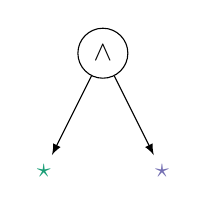
\begin{tikzpicture}[edge from parent/.style={draw,-latex},baseline=(current bounding box.center)]
    \node[draw,circle] {$\land$}
    child {node {\color{color1} $\star$}}
    child {node {\color{color2} $\star$}}
    ;
  \end{tikzpicture},
  \qquad
  L = \langle {\color{color1} \eqref{eq:1}}, {\color{color2} \eqref{eq:2} \land \eqref{eq:3}} \rangle
  \]
  %% Later, both \structure{$G$} and \structure{$L$} are incorporated into a larger \alert{search state}.
\end{frame}
% stars mark edges to nowhere and they are associated with the formulas in L via a certain order

\begin{frame}
  \frametitle<1>{New Rule 1/3: Generalised Domain Recursion}
  \frametitle<2>{New Rule 2/3: Constraint Removal}
  \frametitle<3>{New Rule 3/3: Identifying Possibilities for Recursion}
  \begin{columns}
    \begin{column}{0.15\textwidth}
      \centering
      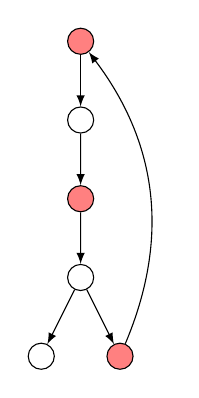
\begin{tikzpicture}[every node/.style={draw,ellipse},edge from parent/.style={draw,-latex},sibling distance=10mm,level distance=10mm]
        \node[fill=red!50, fill on=<1>] (dr) {}
        child {node {}
          child {node[fill=red!50, fill on=<2>] {}
            child {node {}
              child {node {}}
              child {node[fill=red!50, fill on=<3>] (ref) {}}
            }}};
        \draw[-latex, bend right,alt=<3>{red}{black}] (ref) to (dr);
      \end{tikzpicture}
    \end{column}
    \begin{column}{0.85\textwidth}
      \begin{overprint}
        \onslide<1>
          \begin{example}
            Input formula:
            \[
              \forall x \in \Gamma\text{. }\forall y, z \in \Delta\text{. }y \ne z \Rightarrow \neg \pP{}(x, y) \lor \neg \pP{}(x, z)
            \]
            Output formula (with a new constant \structure{$c \in \Gamma$}):
            \begin{gather*}
              \forall y, z \in \Delta\text{. }y \ne z \Rightarrow \neg \pP{}(\alert{c}, y) \lor \neg \pP{}(\alert{c}, z) \\
              \begin{multlined}
                \forall x \in \Gamma\text{. }\forall y, z \in \Delta\text{. }\alert{x \ne c} \land y \ne z \Rightarrow \\
                \neg \pP{}(x, y) \lor \neg \pP{}(x, z)
              \end{multlined}
            \end{gather*}
            %% Output FCG:
            %% \begin{tikzpicture}[edge from parent/.style={draw,-latex}]
            %%   \node[draw,circle] {$\textsc{DR}$}
            %%   child {node {$\star$}}
            %%   ;
            %% \end{tikzpicture}
            %% Here, domain recursion is applied to domain \structure{$M$}. It could similarly be applied to \structure{$N$} as well.
          \end{example}
        \onslide<2>
          \begin{example}
            Input formula (with a constant \structure{$c \in \Gamma$}):
            \begin{gather*}
              \begin{multlined}
                \forall x \in \alert{\Gamma}\text{. }\forall y, z \in \Delta\text{. }\alert{x \ne c} \land y \ne z \Rightarrow \\
                \neg \pP{}(x, y) \lor \neg \pP{}(x, z)
              \end{multlined} \\
              \begin{multlined}
                \forall w,x \in \alert{\Gamma}\text{. }\forall y \in \Delta\text{. }\alert{w \ne c} \land \alert{x \ne c} \land w \ne x \Rightarrow \\
                \neg \pP{}(w, y) \lor \neg \pP{}(x, y)
              \end{multlined}
            \end{gather*}
            Output formula (with a new domain \structure{$\Gamma' \coloneqq \Gamma \setminus \{\, c \,\}$}):
            \begin{gather*}
              \forall x \in \alert{\Gamma'}\text{. }\forall y, z \in \Delta\text{. }y \ne z \Rightarrow \neg \pP{}(x, y) \lor \neg \pP{}(x, z) \\
              \forall w,x \in \alert{\Gamma'}\text{. }\forall y \in \Delta\text{. }w \ne x \Rightarrow \neg \pP{}(w, y) \lor \neg \pP{}(x, y)
            \end{gather*}
          \end{example}
        \onslide<3>
          \begin{block}{Goal}
            Check if the input formula is equivalent (up to domains) to a
            previously encountered formula.
          \end{block}
          \begin{block}{Rough Outline}
            \begin{enumerate}
              \item Consider pairs of `similar' clauses.
              \item Consider bijections between their sets of variables.
              \item Extend each such bijection to a map between sets of domains.
              \item If the bijection makes the clauses equal, and the domain map
                    is compatible with previous domain maps, move on to another
                    pair of clauses.
            \end{enumerate}
          \end{block}
      \end{overprint}
    \end{column}
  \end{columns}
\end{frame}
% We're still creating a vertex in a graph with one outgoing edge.

%% \begin{frame}{Compilation as Search}
%%   \begin{definition}
%%     A \alert{(search) state} is a tuple \structure{$(G, C, L)$}, where:
%%     \begin{itemize}
%%     \item \structure{$G$} is an FCG (or \texttt{null}),
%%     \item \structure{$C$} is a compilation cache that maps integers to sets of pairs $(\phi, v)$, where $\phi$ is a formula, and $v$ is a vertex of $G$ (which is used to identify opportunities for recursion),
%%     \item and \structure{$L$} is a list of formulas (that are yet to be compiled). (Note that the order is crucial!)
%%     \end{itemize}
%%   \end{definition}
%%   The search algorithm combines greedy and breadth-first search:
%% \end{frame}

\begin{frame}{Resulting Improvements to Counting Functions}
  Let \structure{$\Gamma$} and \structure{$\Delta$} be two sets with
  cardinalities \structure{$|\Gamma| = m$} and \structure{$|\Delta| = n$}.

  Our new compilation rules enables us to count \structure{$\Gamma \to \Delta$}
  functions such as: \vspace{1em}
  \begin{itemize}
    \item injections in \structure{$\Theta(mn)$} time
          \begin{itemize}
            \item by hand: \structure{$\Theta(m)$}
          \end{itemize}
    \item partial injections in \structure{$\Theta(mn)$} time
          \begin{itemize}
            \item by hand: \structure{$\Theta({\min\{\, m, n \,\}}^2)$}
          \end{itemize}
          \item bijections in \structure{$\Theta(m)$} time
          \begin{itemize}
            \item \alert{optimal!}
          \end{itemize}
  \end{itemize}
\end{frame}

\begin{frame}{Summary \& Future Work}
  \begin{block}{Summary}
    The circuits hitherto used for FOMC become more powerful with:
    \begin{itemize}
    \item cycles,
    \item generalised domain recursion,
    \item and some more new compilation rules that support domain recursion.
    \end{itemize}
  \end{block}
  \begin{block}{Future Work}
    \begin{itemize}
    \item Automate:
      \begin{itemize}
      \item simplifying the definitions of functions,
      \item finding all base cases.
      \end{itemize}
    \item Open questions:
      \begin{itemize}
      \item What kind of \alert{sequences} are computable in this way?
      \item Would using a \alert{different logic} extend the capabilities of FOMC further?
      \end{itemize}
    \end{itemize}
  \end{block}
\end{frame}

\end{document}
